%----------------------------------------------------------------------------------------
%	PACKAGES AND THEMES
%----------------------------------------------------------------------------------------
\documentclass[aspectratio=169,xcolor=dvipsnames,t]{beamer}
\usetheme{SimplePlus}
\usepackage{amsmath}
\usepackage{amssymb}
\usepackage{mathtools}
\usepackage{amsfonts}
\usepackage{tikz}
\usepackage{caption}
\usepackage{subcaption}
\usepackage[export]{adjustbox}
\usepackage[shortlabels]{enumitem}
\usepackage{hyperref}
\usepackage{graphicx} % Allows including images
\usepackage{booktabs}
\usepackage{emoji}
\usepackage{cancel}
\usepackage{algorithm2e}
\usepackage{algorithmic}
\usepackage{float}
\usepackage{pst-tree}
\usepackage{forest}
\usepackage{makecell}
\usepackage{ragged2e}
\psset{treemode=D,nodesep=3pt}\usepackage{lmodern}
\usetikzlibrary{decorations.pathreplacing, positioning}

\DeclareMathOperator*{\expectation}{\mathbb{E}}
\DeclareMathOperator*{\looongrightarrow}{%
  \DOTSB\relbar\joinrel\relbar\joinrel\relbar\joinrel\relbar\joinrel\relbar\joinrel\relbar\joinrel\relbar\joinrel\relbar\joinrel\relbar\joinrel\rightarrow
}

%----------------------------------------------------------------------------------------
%	TITLE PAGE
%----------------------------------------------------------------------------------------

\title[short title]{From external to swap regret 2.0} % The short title appears at the bottom of every slide, the full title is only on the title page
\subtitle{An Efficient Reduction for Large Action Spaces}

\author{Shahar Glam \and Daniel Volkov}

\institute[TAU] % Your institution as it will appear on the bottom of every slide, may be shorthand to save space
{
    Tel-Aviv University  % Your institution for the title page
}
\date{December 9, 2024} % Date, can be changed to a custom date


%----------------------------------------------------------------------------------------
%	PRESENTATION SLIDES
%----------------------------------------------------------------------------------------

\begin{document}
\setemojifont{AppleColorEmoji.ttf}


\begin{frame}
    \titlepage
\end{frame}

\begin{frame}{Authors}
    \vfill\null
    \begin{figure}[h]
        \centering
        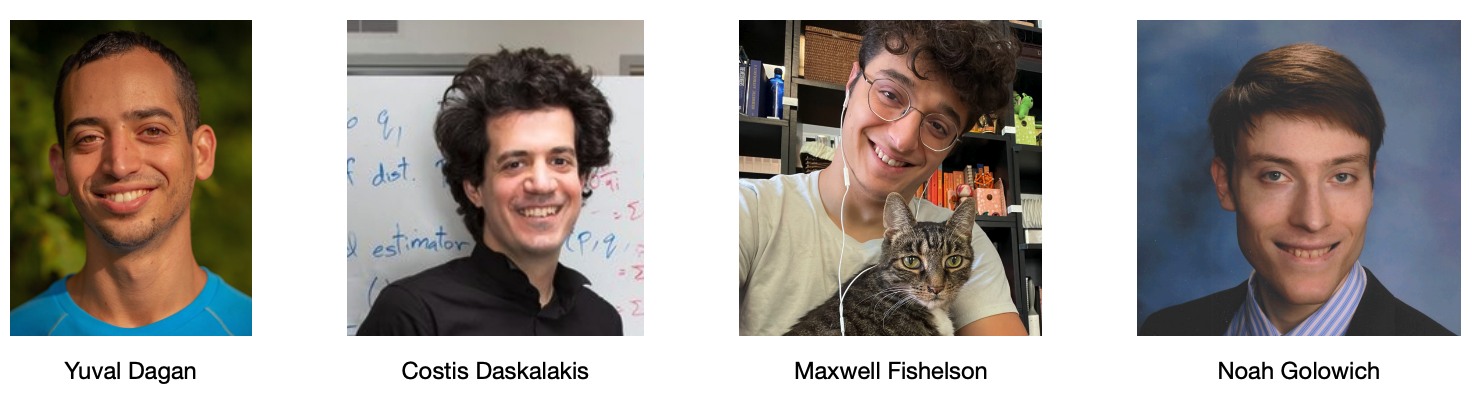
\includegraphics[width=1\linewidth]{Screenshot 2024-12-06 at 17.29.21.png}
    \end{figure}
    \vfill\null
\end{frame}

\begin{frame}[label=last]{Overview}
    \tableofcontents
\end{frame}

%------------------------------------------------
\section{Introduction}
%------------------------------------------------
% \begin{frame}{What Is Game Theory?}
%     \begin{definition}[Oxford]
%         "the branch of mathematics
%         concerned with the analysis of strategies for dealing with competitive
%         situations where the outcome of a participant’s choice of action
%         depends critically on the actions of other participants"
%     \end{definition}
%     \begin{columns}[c]
%     \column{.65\textwidth}  
%     \begin{definition}[Myerson] 
%         "the study of
%         mathematical models of conflict and cooperation
%         between intelligent rational decision-makers"
%     \end{definition}
%     \column{.3\textwidth}
%         \begin{figure}
%         \centering
%         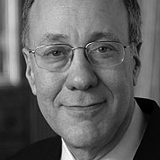
\includegraphics[width=0.4\linewidth]{myerson.png}
%         \label{fig:Myerson-pic}
%         \end{figure}
%     \end{columns}

%     % Explain the problem at hand: we have a game setting and want to find equilibrium\\
%     % what is a game? what is equilibrium? here just motivation and intuition 
% \end{frame}

\begin{frame}{Example - The Prisoner's Dilemma}
    \begin{example}[Prisoner's Dilemma]
        \begin{enumerate}[$\bullet$]
            \item Two bank robbers are arrested and being interrogated.
            \item Police only has evidence of minor offenses.
            \item The robbers are interrogated separately and can't communicate with each other.
            \item Each robber can either cooperate with the police \emoji{rat} or remain silent \emoji{zipper-mouth-face}.
        \end{enumerate}
    \end{example}
    \pause
    \begin{table}
        \centering
        \begin{tabular}{|c||c|c|}
            \hline
            $_{A_1}\backslash^{A_2}$ & \emoji{rat}_2 & \emoji{zipper-mouth-face}_2 \\ 
            \hline\hline
            \emoji{rat}_1 & $(-5,-5)$ & $(0,-20)$ \\
            \emoji{zipper-mouth-face}_1 & $(-20,0)$ & $(-1,-1)$ \\
            \hline
        \end{tabular}
        \label{tab:RPCPrisonDillema}
    \end{table}
    % NOTES: Explain the settings and the dillema.
\end{frame}

%------------------------------------------------
\section{Preliminaries}
\subsection{Strategic game setting}
%------------------------------------------------

\begin{frame}{Strategic game setting}
    \begin{definition}[Strategic game]
        A strategic game is a triplet $\langle K,A, f\rangle$, where $A =\bigtimes_{i=1}^K A_i$ is the set of all player's actions, and $f = (f_1,\dots,f_K):A\rightarrow\mathbb{R}^K$ is the payoff (or reward) function.
    \end{definition}
    \alt<1-6>{\begin{columns}
    \pause
    \column{.4\textwidth}
    \begin{center}
    A \color{blue} normal form \color{black} game
        \begin{table}
            \centering
            \begin{tabular}{|c||c|c|c|}
                \hline
                $_{A_1}\backslash^{A_2}$ & \emoji{rock}_2 & \emoji{page-facing-up}_2 & \emoji{scissors}_2 \\ 
                \hline\hline
                \emoji{rock}_1 & $(0,0)$ & $(-1,1)$ & $(1,-1)$ \\
                \emoji{page-facing-up}_1 & $(1,-1)$ & $(0,0)$ & $(-1,1)$ \\
                \emoji{scissors}_1 & $(-1,1)$ & $(1,-1)$ & $(0,0)$ \\
                \hline
            \end{tabular}
            \label{tab:normalFormGameExample}
        \end{table}
    \end{center}
    \pause
    \column{.6\textwidth}
        \begin{center}
            $K=2$ \pause \\
            $A_i$=\{\emoji{rock}$_i$,\emoji{page-facing-up}$_i$,\emoji{scissors}$_i$\}\\ \pause
            $A=$\{(\emoji{rock},\emoji{rock}),(\emoji{page-facing-up},\emoji{page-facing-up}), \\
            $\text{(\emoji{scissors},\emoji{scissors}), (\emoji{rock},\emoji{scissors}), (\emoji{scissors},\emoji{rock}),} \dots \}$ \pause
            $f(\text{\emoji{rock},\emoji{rock})$=$f(\emoji{scissors},\emoji{scissors})$=$f(\emoji{page-facing-up},\emoji{page-facing-up})$=(0,0)$},\dots$ \pause
        \end{center}
    \end{columns}}
    {\begin{Definition}[Strategy profile]
        $s = (s_i;s_{-i}) =(s_1,\dots,s_n) \in A$ is called a strategy profile, where $s_i\in A_i$ is the strategy (or action) of player $i$
    \end{Definition}}
\end{frame}

%------------------------------------------------
\subsection{Types of equilibrium}
%------------------------------------------------

\begin{frame}{Equilibrium}
    \begin{alertblock}{Game Equilibrium}
        Strategy profile where no player wants to deviate
    \end{alertblock}
    \begin{columns}
        \column{0.3\textwidth}
        \centering
        \tikzset{set/.style={draw,circle,inner sep=0pt,align=center}}
        \only<2->{\begin{tikzpicture}
            \node[set,fill=green!20,text width=20pt]{A};
        \end{tikzpicture}}
        \only<1->{{\huge\emoji{thinking}}}\\ 
        \only<4->{\vspace{20} \textbf{Coarse Deviations}
        \begin{table}[]
            \centering
            \begin{tabular}{c|c}
                \begin{tikzpicture}
                    \node[set,fill=green!20,text width=20pt]{A};
                \end{tikzpicture} & \begin{tikzpicture}
                    \node[set,fill=red!20,text width=20pt]{Z};
                \end{tikzpicture}\\
                \begin{tikzpicture}
                    \node[set,fill=green!20,text width=20pt]{B};
                \end{tikzpicture} & \begin{tikzpicture}
                    \node[set,fill=red!20,text width=20pt]{Z};
                \end{tikzpicture}\\
                \begin{tikzpicture}
                    \node[set,fill=green!20,text width=20pt]{C};
                \end{tikzpicture} & \begin{tikzpicture}
                    \node[set,fill=red!20,text width=20pt]{Z};
                \end{tikzpicture}
            \end{tabular}
            \label{tab:my_label}
        \end{table}}
        \column{0.3\textwidth}
        \centering
        \tikzset{set/.style={draw,circle,inner sep=0pt,align=center}}
        \only<2->{\begin{tikzpicture}
            \node[set,fill=green!20,text width=20pt]{B};
        \end{tikzpicture}}
        \only<1->{{\huge\emoji{thinking}}}\\ \vspace{20}
        \only<5->{\textbf{Swap Deviations}
        \begin{table}[]
            \centering
            \begin{tabular}{c|c}
                \begin{tikzpicture}
                    \node[set,fill=green!20,text width=20pt]{A};
                \end{tikzpicture} & \begin{tikzpicture}
                    \node[set,fill=green!20,text width=20pt]{A};
                \end{tikzpicture}\\
                \begin{tikzpicture}
                    \node[set,fill=green!20,text width=20pt]{B};
                \end{tikzpicture} & \begin{tikzpicture}
                    \node[set,fill=green!20,text width=20pt]{B};
                \end{tikzpicture}\\
                \begin{tikzpicture}
                    \node[set,fill=green!20,text width=20pt]{C};
                \end{tikzpicture} & \begin{tikzpicture}
                    \node[set,fill=red!20,text width=20pt]{Z};
                \end{tikzpicture}
            \end{tabular}
            \label{tab:my_label}
        \end{table}}
        \column{0.3\textwidth}
        \centering
        \tikzset{set/.style={draw,circle,inner sep=0pt,align=center}}
        \only<2->{\begin{tikzpicture}
            \node[set,fill=green!20,text width=20pt]{C};
        \end{tikzpicture}}
        \alt<1-2>{{\huge\emoji{thinking}}}{{\huge\reflectbox{\emoji{thinking}}}}
        \only<3->{\begin{tikzpicture}
            \node[set,fill=red!20,text width=20pt]{Z};
        \end{tikzpicture}}\\ \vspace{20}
        \only<6->{\textbf{CCE:} No player wants to make a coarse deviation\\
        \textbf{CE:} No player wants to make a swap deviation\\
        \textbf{NE:} No player wants to make a swap deviation \color{red} AND \color{black} profile must be independent}
    \end{columns}
\end{frame}

%------------------------------------------------
%------------------------------------------------

\begin{frame}{Nash Equilibrium}
    \begin{definition}[Nash equilibrium]
        A strategy profile $s^*$ in a game $\langle K,A,f\rangle$ is called a \textbf{Nash equilibrium} if for all $i\in [K]$:
        \begin{equation*}
            \forall d\in A_i:\; f_i(s^*_i;s^*_{-i}) \geq f_i(d;s^*_{-i})
        \end{equation*}
    \end{definition}
    \pause
    \begin{table}
        \centering
        \begin{tabular}{|c||c|c|}
            \hline
            $_{A_1}\backslash^{A_2}$ & \emoji{pizza}_2 & \emoji{hamburger}_2 \\ 
            \hline\hline
            \emoji{pizza}_1 &\only<2>{$(2,1)$}
            \only<3>{\fcolorbox{MediumRed}{InvisibleRed}{$(2,1)$}} & $(0,0)$ \\
            \emoji{hamburger}_1 & $(0,0)$ & \only<2>{$(1,2)$}\only<3>{\fcolorbox{MediumRed}{InvisibleRed}{$(1,2)$}} \\
            \hline
        \end{tabular}
        \label{tab:RPCPrisonDillema}
    \end{table}
\end{frame}

%------------------------------------------------
%------------------------------------------------

\begin{frame}[label=current]{Correlated Equilibrium (CE)}
    \begin{definition}[Correlated equilibrium]
        Let $Q$ be a \textbf{distribution} over $A$. $Q$ is called a Correlated equilibrium, if for all $i\in [K]$, and for every function $\phi:A_i\rightarrow A_i$:
        \begin{equation*}
            \expectation_{s\sim Q}[f_i(s)] \geq \expectation_{s\sim Q}[f_i(\phi(s_i);s_{-i})]
        \end{equation*}
    \end{definition}\pause
    \only<2>{\begin{Definition}[$\varepsilon$-approximate-CE]
    $Q$ is called an $\varepsilon$-Correlated equilibrium if for all $i\in [K]$, and for every function $\phi:A_i\rightarrow A_i$:
    \begin{equation*}
        \varepsilon + \expectation_{s\sim Q}[f_i(s)] \geq \expectation_{s\sim Q}[f_i(\phi(s_i);s_{-i})]
    \end{equation*}
    \end{Definition}}
    \pause
        \begin{columns}[c]
            \column{.55\textwidth} 
            \begin{table}
                \centering
                \begin{tabular}{|c||c|c|}
                    \hline
                    $_{A_1}\backslash^{A_2}$ & \emoji{automobile}\emoji{dashing-away}_2 & \emoji{stop-sign}_2  \\ 
                    \hline\hline
                    \emoji{automobile}\emoji{dashing-away}_1 & $(-100,-100)$ & \alt<4->{\fcolorbox{MediumRed}{InvisibleRed}{$(0,-1)$}}{$(0,-1)$}\\
                    \emoji{stop-sign}_1 & \alt<4->{\fcolorbox{MediumRed}{InvisibleRed}{$(-1,0)$}}{$(-1,0)$} & $(-1,-1)$  \\
                    \hline
                \end{tabular}
                \label{tab:ChickenGameExample}
            \end{table}
            \column{.4\textwidth}
            \only<5>{
            \begin{center}
                \textbf{Correlated Equilibrium:}
                $p(S,C) = \frac{1}{2}, p(C,S)=\frac{1}{2}, $
                $p(C,C)=p(S,S) = 0$
            \end{center}}
        \end{columns}    
\end{frame}

%------------------------------------------------
%------------------------------------------------

\begin{frame}{Coarse Correlated Equilibrium (CCE)}
    \begin{definition}[Coarse Correlated equilibrium]
        Let $Q$ be a \textbf{distribution} over $A$. $Q$ is called a Coarse Correlated equilibrium, if for all $i\in [K]$ ,and for all $d\in A_i$:
        \begin{equation*}
            \expectation_{s\sim Q}[f_i(s)] \geq \expectation_{s\sim Q}[f_i(d;s_{-i})]
        \end{equation*}
    \end{definition}
    \begin{Definition}[$\varepsilon$-CCE]
    $Q$ is called an $\varepsilon$-Coarse Correlated equilibrium if for all $i\in [K]$, and for all $d\in A_i$:
    \begin{equation*}
        \varepsilon + \expectation_{s\sim Q}[f_i(s)] \geq \expectation_{s\sim Q}[f_i(d;s_{-i})]
    \end{equation*}
    \end{Definition}
\end{frame}

%------------------------------------------------
%------------------------------------------------

\begin{frame}{CE VS CCE}
    \begin{columns}
        \column{.5\textwidth}
        \begin{definition}[Correlated equilibrium]
            \begin{equation*}
                \forall \phi:A_i\rightarrow A_i:\; \expectation_{s\sim Q}[f_i(s)] \geq   \expectation_{s\sim Q}[f_i(\phi(s_i);s_{-i})]
            \end{equation*}
        \end{definition}
        
        \column{.5\textwidth}
        \begin{definition}[Coarse Correlated equilibrium]
            \begin{equation*}
                \forall d\in A_i:\; \expectation_{s\sim Q}[f_i(s)] \geq \expectation_{s\sim Q}[f_i(d;s_{-i})]
            \end{equation*} 
        \end{definition}
        
    \end{columns}
    \begin{columns}
        \column{.6\textwidth}
        \only<2->{{\begin{table}
            \centering
            \begin{tabular}{|c||c|c|c|}
                \hline
                $_{A_1}\backslash^{A_2}$ & A & B & C \\ 
                \hline\hline
                A & $(1,-1)$ & $(-1,1)$ & $(-\infty,-\infty)$ \\
                B & $(-1,1)$ & $(1,-1)$ & $(-\infty,-\infty)$ \\
                C & $(-\infty,-\infty)$ & $(-\infty,-\infty)$ & \alt<3->{\fcolorbox{MediumRed}{InvisibleRed}{$(-10,-10)$}}{$(-10,-10)$} \\
                \hline
            \end{tabular}
            \label{tab:AllEquilibriaExample}
        \end{table}}}
        \column{.4\textwidth}
        \begin{center}
            \only<4->{
                \color{MediumRed}\textbf{CE}\color{black} \\
                $P(A,B)=P(B,A)=$\\
                $P(A,A)=P(B,B)=\frac{1}{8}$ \\
                $P(C,C) = \frac{1}{2}$ \\
            }
            \only<5->{
                \color{MediumRed}\textbf{CCE}\color{black} \\
                $P(A,A)=P(C,C)=\frac{1}{2}$ \\
            }
        \end{center}
    \end{columns}
\end{frame}
%------------------------------------------------
%------------------------------------------------

\begin{frame}{Hierarchy Of Equilibrium}
\centering
\tikzset{set/.style={draw,circle,inner sep=0pt,align=center}}
\begin{center}
\begin{tikzpicture}
    \node[set,fill=MediumGreen!20,text width=5cm,label={[below=10pt of rea,text opacity=1]CCE}] 
      (nat) at (0,0.7)  (rea) {};
    \node[set,fill=blue!20,text width=4cm,label={[below=8pt of rea]CE}] 
      (int) at (0,0.3)  (int){};
    \node[set,fill=MediumRed!20,text width=2.5cm] (nat) at (0,0) {NE};
\end{tikzpicture}
\end{center}
\end{frame}

%------------------------------------------------
\subsection{Online learning setting}
%------------------------------------------------

\begin{frame}{Online learning setting}
    A \textbf{single player} plays against an adversary for $T$ rounds trying to maximize their \textbf{reward}.\\
    In each round $t = 1,...,T$:\\
    \begin{enumerate}[$\bullet$]
        \pause\item The player picks a probability distribution $x^{(t)}=(x_1^{(t)},...,x_N^{(t)})$ over $A$.
        \pause\item The adversary picks a reward vector $f^{(t)} = (f_1^{(t)},\dots,f_N^{(t)})\in [0,1]^N$.
        \pause\item 
            The player achieves $x^{(t)}\cdot f^{(t)}$ reward at round $t$.
    \end{enumerate}
\end{frame}

%------------------------------------------------
%------------------------------------------------

\begin{frame}[label=current]{Regret in online learning}
    \begin{alertblock}{Regret}
        The difference between the obtained reward and a benchmark
    \end{alertblock}
    \begin{columns}
        \pause \column{.4\textwidth}
        \begin{equation*}
            \sum_{t=1}^T x^{(t)}\cdot f^{(t)}
        \end{equation*}
        \pause \column{.2\textwidth}
        \begin{equation*}
            \looongrightarrow_{\text{Benchmark: best }\phi\in \Phi}
        \end{equation*}
        \column{.4\textwidth}
        \begin{equation*}
            \sum_{t=1}^T \phi(x^{(t)})\cdot f^{(t)}
        \end{equation*}
    \end{columns}
    \pause
    \vspace{0.4cm}
    $\bullet$ Where $\Phi$ is a set of transformations $\phi:\Delta_N\rightarrow\Delta_N$\\
    \pause
    \begin{definition}[Regret against $\Phi$]
        The regret of an online learner is defined as:
        \begin{equation*}
            \text{Regret}_{\Phi}(x^{(1:T)};f^{(1:T)}) = \left(\max_{\phi\in\Phi} \sum_{t=1}^T \phi(x^{(t)})\cdot f^{(t)}\right) - \sum_{t=1}^T x^{(t)}\cdot f^{(t)}
        \end{equation*}
    \end{definition}
\end{frame}

%------------------------------------------------
\subsection{Types of regret}
%------------------------------------------------

\begin{frame}[label=current]{Swap Regret}
    \begin{definition}[Swap Regret]
        The \color{MediumRed} swap regret \color{black} of an online learner is defined as the regret against the set of \textbf{all maps}. namely:
        \begin{equation*}
            \text{SR}(x^{(1:T)};f^{(1:T)}) = \left(\max_{\phi:\Delta_N\rightarrow\Delta_N} \sum_{t=1}^T \phi(x^{(t)})\cdot f^{(t)}\right) - \sum_{t=1}^T x^{(t)}\cdot f^{(t)}
        \end{equation*}
    \end{definition}
    \pause
    
    \begin{theorem}[$\varepsilon$-SR induces an $\varepsilon$-CE]
        If each player achieves swap regret bounded above by $\varepsilon$, then the joint distribution of all player actions is an $\varepsilon$-Correlated equilibrium.
    \end{theorem}
    \pause
    
    $\bullet$ \textbf{Proof sketch}: for each player, the maximum over all maps is at least as big as over a \color{MediumGreen}swap function\color{black}. If we now define the same swap on the distribution, we get the definition of $\varepsilon$-CE.
\end{frame}
%------------------------------------------------
%------------------------------------------------

\begin{frame}[label=current1]{$\varepsilon$-SR induces an $\varepsilon$-CE}
    Assume each player achieves swap-regret bounded by $\varepsilon$. \pause
    namely $\forall i\in$ [K] and $\forall\phi^*:\Delta_N\rightarrow\Delta_N$:
    \begin{equation*}
        \expectation_{s\sim \phi^*(X)}[f_i(s)] - \expectation_{s\sim X}[f_i(s)]\leq\left(\max_{\phi:\Delta_N\rightarrow\Delta_N}\sum_{t=1}^T \phi(x^{(t)})\cdot f^{(t)}\right)-\sum_{t=1}^T x^{(t)}\cdot f^{(t)}\leq \varepsilon
    \end{equation*}
    \pause
    Let $\phi:A_i\rightarrow A_i$ be a swap function. Define $\hat{\phi}:\Delta_N\rightarrow\Delta_N$ such that $x\sim X \iff \phi(x)\sim\hat{\phi}(X)$.\\
    \pause We have:
    \begin{equation*}
        \expectation_{s\sim X}[f_i(\phi(s_i);s_{-i})]-\expectation_{s\sim X}[f_i(s)]=\expectation_{s\sim \hat{\phi}(X)}[f_i(s)] - \expectation_{s\sim X}[f_i(s)] \leq \varepsilon
    \end{equation*}
    
\end{frame}

%------------------------------------------------
%------------------------------------------------

\begin{frame}{External regret}
    \begin{definition}[External regret]
        The \color{MediumRed} external regret \color{black} of an online learner is defined as the regret against the set of all \textbf{constant maps}. (Map $x^{(t)}$ to a distribution where $\exists i\in [N]:P(i)=1$)\\
        Namely:
        \begin{equation*}
            \text{ER}(x^{(1:T)};f^{(1:T)}) = \left(\max_{i\in [N]}\sum_{t=1}^T f_i^{(t)}  \right) - \sum_{t=1}^Tx^{(t)}\cdot f^{(t)}
        \end{equation*}
    \end{definition}
    \pause
    \begin{itemize}[\bullet]
        \item 
            External regret minimization is a much(\emoji{double-exclamation-mark}) easier task then swap regret minimization
        \pause
        \item
            This is enough to guarantee swap regret minimization! (\textit{foreshadowing}\emoji{cook-light-skin-tone})
    \end{itemize}
\end{frame}

%------------------------------------------------
\subsection{No-regret learning}
%------------------------------------------------

\begin{frame}[label=current]{No-external-regret learning}
    \only<1-7>{
        \begin{alertblock}{Multiplicative Weight Updates}
            Look at the past, do the best thing (with some normalization)
        \end{alertblock}
    }
    \only<8->{
        \begin{alertblock}{\textbf{Lazy} Multiplicative Weight Updates}
            Look at the past, do the best thing (with some normalization) \textbf{Every B rounds}
        \end{alertblock}
    }
    \begin{columns}
        \column{0.4\textwidth}
            \only<2->{\centering $F^{(t)} \vcentcolon = \frac{1}{t}\sum_{i=1}^t f^{(i)}$}
            \only<3-7>{\begin{table}[h]
                \centering
                \begin{tabular}{c|c}
                     Rewards & Actions \\ \hline
                     \only<3-7>{$F^{(0)}$} & \only<4-7>{$x^{(1)} = $ softmax$(\eta \cdot F^{(0)})$} \\
                     \only<5-7>{$F^{(1)}$} & \only<6-7>{$x^{(2)} = $ softmax$(\eta \cdot F^{(1)})$} \\
                     \only<7>{$F^{(2)}$} & \only<7>{$x^{(3)} = $ softmax$(\eta \cdot F^{(2)})$} \\
                     \only<7>{$F^{(3)}$} & \only<7>{$x^{(4)} = $ softmax$(\eta \cdot F^{(3)})$} \\
                     \only<7>{$F^{(4)}$} & \only<7>{$x^{(5)} = $ softmax$(\eta \cdot F^{(4)})$} \\
                \end{tabular}
                \label{tab:my_label}
            \end{table}}
            \only<8->{\begin{table}[h]
                \centering
                \begin{tabular}{c|c}
                     Rewards & Actions \\ \hline
                     \only<8->{$F^{(0)}$} & \only<9->{$x^{(1)} = $ softmax$(\eta \cdot F^{(0)})$} \\
                     \only<10->{$F^{(1)}$} & \only<11->{\color{MediumRed}$x^{(2)} = $ softmax$(\eta \cdot F^{(0)})$\color{black}} \\
                     \only<12->{$F^{(2)}$} & \only<13->{$x^{(3)} = $ softmax$(\eta \cdot F^{(2)})$} \\
                     \only<14->{$F^{(3)}$} & \only<14->{\color{MediumRed}$x^{(4)} = $ softmax$(\eta \cdot F^{(2)})$\color{black}} \\
                     \only<14->{$F^{(4)}$} & \only<14->{$x^{(5)} = $ softmax$(\eta \cdot F^{(4)})$} \\
                \end{tabular}
                \label{tab:my_label}
            \end{table}}
        \only<15->{\column{0.6\textwidth}
        \begin{center}
            
            \begin{tikzpicture}[
                every node/.style={font=\small},
                box/.style={draw, minimum height=1cm, minimum width=1cm, align=center}
            ]
            
            % Draw the main rectangle
            \only<15->{\draw[thick] (0,0) rectangle (7.5,1);}
            
            % Vertical lines for segments
            \only<16->{\foreach \x in {1.5,3,4.5,6} {
                \draw[MediumRed, thick] (\x,0) -- (\x,1);
            }}
            \only<16-17>{
                \node at (0.75,0.5) {$1$};
                \node at (2.25,0.5) {$2$};
                \node at (3.75,0.5) {$3$};
                \node at (5.25,0.5) {$\dots$};
                \node at (6.75,0.5) {$M$};    
            }
            
            % Labels inside the segments
            \only<19->{\node at (0.75,0.5) {$x^{(1)}\ x^{(1)}$};}
            \only<21->{\node at (2.25,0.5) {$x^{(B)}\; x^{(B)}$};}
            \only<23->{\node at (3.75,0.5) {$x^{(2B)} x^{(2B)}$};}
            \only<24->{\node at (5.25,0.5) {$x^{(3B)}x^{(3B)}$};
            \node at (6.75,0.5) {$\cdots$};}
            
            % U labels below the boxes
            \only<18->{\node[below] at (0,0) {$F^{(0)}$};}
            \only<20->{\node[below] at (1.5,0) {$F^{(B)}$};}
            \only<22->{\node[below] at (3,0) {$F^{(2B)}$};}
            \only<24->{\node[below] at (4.5,0) {$F^{(3B)}$};}
            
            % T label above the rectangle
            \only<15-16>{\node[above right] at (7.5,1) {$T$};}
            \only<17->{\node[above right] at (7,1) {$T = BM$};}
            
            \node[above left] at (0,1) {$0$};
            
            \end{tikzpicture}
            \vfill\null
            \only<25->{MWU: $\varepsilon$-ER for $T=\Omega \left(\frac{\log N}{\varepsilon^2}\right)$} \\
            
            \only<26->{\color{MediumRed}Lazy \color{black} MWU: $\varepsilon$-ER for $\color{MediumRed}M\color{black}=\Omega\left(\frac{\log N}{\varepsilon^2}\right)$
            }
        \end{center}}
    \end{columns}
\end{frame}

\section{From external to swap regret}
\subsection{Blum-Mansour algorithm}

%------------------------------------------------
\begin{frame}[label=last]{Blum-Mansour algorithm}
\begin{columns}
    \column{0.5\textwidth}
        \begin{tikzpicture}
            \newcommand{\height}{4}
            \draw[thick] (0,0) rectangle (1,1) 
            \node at (0.5,0.5) {$B_N$}
            \draw[thick] (0,\height) rectangle ++(1,1) 
            \node at (0.5,\height + 0.5) {$B_1$}
            \node at (0.5,\height/2 + 0.5) {\vdots}
            \pause \draw [->] (1.1,.8) -- node[above=.1mm] {$q_N^{(t)}$} ++(2.8,0);
            \draw [<-] (1.1,0) -- node[above=.1mm] {$f_N^{(t)}$} ++(2.8,0);
            \draw [->] (1.1,\height + .8) -- node[above=.1mm] {$q_1^{(t)}$} ++(2.8,0);
            \draw [<-] (1.1,\height) -- node[above=.1mm] {$f_1^{(t)}$} ++(2.8,0);
            \pause\filldraw[color=blue!60, fill=blue!5, thick] (4,0) rectangle ++(.6, \height + 1) 
            \draw [->] (4.6,\height/2 + .8) -- node[above=.1mm] {$p^{(t)}$} ++(1.8,0);
            \draw [<-] (4.6,\height/2) -- node[above=.1mm] {$f^{(t)}$} ++(1.8,0);
        \end{tikzpicture}
    \column{0.5\textwidth}
        \only<4->{
            \begin{enumerate}[i)]
                \only<4->{\item 
                    Calculating $p^{(t)}$ from $\vec{q}_1^{(t)}, \dots, \vec{q}_N^{(t)}$.}
                \only<5->{\item 
                    Distributing the reward across the algorithms $B_1,\dots, B_N$.}
            \end{enumerate}
        }
\end{columns}
\end{frame}

\begin{frame}{Blum-Mansour algorithm}
    \textbf{Distribute}: $B_i$ \leftarrow $f^{(t)}_i=f^{(t)}\cdot p^{(t)}_i$\\
    \pause \textbf{Calculate p:} \big{\textbf{LATER!}}\\
    \pause Denote:
    \begin{equation*}
        Q = \begin{pmatrix}
            q_{11} & \dots & q_{1N} \\
            \vdots & \ddots & \vdots \\
            q_{N1} & \dots & q_{NN} \\
        \end{pmatrix} = 
        \begin{pmatrix}
            \vec{q}_{1}^{(t)} \\
            \vdots \\ 
            \vec{q}_{N}^{(t)} 
        \end{pmatrix}
    \end{equation*}\\
    \pause $F^{(t)} \vcentcolon= \text{Alg reward at time $t$}$\\
    \pause $F^T \vcentcolon = \sum_{i=1}^T F^{(t)}$\\
    \pause $F_{B_i}^{(t)} \vcentcolon = \text{$B_i$ reward at time $t$}$\\
    \pause $F_{B_i}^T \vcentcolon = \sum_{i=1}^T F_{B_i}^{(t)}$\\
\end{frame}

\begin{frame}[label=last]{Proof.}
    $B_i$'s Reward is: $$F_{B_i}^{(t)} = (p_i^{(t)} f^{(t)})\cdot\vec{q}_i^{(t)} = p_i^{(t)} (f^{(t)}\cdot \vec{q}_i^{(t)})$$
    \pause \\ $B_i$ Is a no ER Algorithm!
    \pause $$ \varepsilon + F^T_{B_i} = \varepsilon + \sum_{t=1}^T p_i^{(t)}(\vec{q}_i^{(t)} \cdot f^{(t)})  \geq \sum_{t=1}^T p_i^{(t)} \cdot f^{(t)}_{\phi(j)}$$
    \pause For every $t \in [T]$:
    $$
        \sum_{i=1}^N (p_i^{(t)} \cdot\vec{q}_i^{(t)})f^{(t)}= \sum_{i=1}^N p_i^{(t)}(\vec{q}_i^{(t)}\cdot f^{(t)}) = p^{(t)} Q f^{(t)} =
            \underset{\text{Choose $p=pQ$}}{\underbrace{ p^{(t)} \cdot f^{(t)}}} = F^{(t)}
    $$
    \pause Hence our total reward is:
    $$
        \varepsilon + F^{T} = \varepsilon + \sum_{i=1}^N F_{B_i}^{T} \geq \sum_{i=1}^N \sum_{t=1}^T p_i^{(t)} \cdot f^{(t)}_{\phi(i)}
    $$
\end{frame}
%------------------------------------------------


%------------------------------------------------
%------------------------------------------------

\begin{frame}[label=current]{Tree-Swap}
    \begin{theorem}[From external to swap regret]
        Let $M,d\in\mathbb{N}$, and let $\mathcal{F}$ be a function class.\\
        If there exists a learner for $\mathcal{F}$ that achieves $\varepsilon$ \color{MediumRed}external-regret \color{black} after $M$ rounds, then there is a learner for $\mathcal{F}$ that achieves \color{MediumGreen}swap-regret \color{black} of at most $\varepsilon+\frac{1}{d}$ after $T=M^d$ rounds.
    \end{theorem}
\end{frame}

% %------------------------------------------------
\subsection{Tree-swap algorithm}
\subsection{Proof sketch}
% %------------------------------------------------

\begin{frame}
\frametitle<1-13>{Tree-Swap}
\frametitle<14->{Proof-Sketch}
\begin{columns}[c]
\only<1-26>{
\column{0.6\textwidth} 
\centering
$T=M^d$
\begin{tikzpicture}[level distance=2cm,sibling distance=3cm]
\only<1>{
\tikzstyle{slide2}=[transparent,parent anchor=north, child anchor=south]
}
\only<2->{
\tikzstyle{slide2}=[opaque,parent anchor=south, child anchor=north]
}
\only<1-2>{
\tikzstyle{slide3}=[transparent,parent anchor=north, child anchor=south]
}
\only<3->{
\tikzstyle{slide3}=[opaque,parent anchor=south, child anchor=north]
}
\only<1-3>{
\tikzstyle{slide4}=[transparent,parent anchor=north, child anchor=south]
}
\only<4->{
\tikzstyle{slide4}=[opaque,parent anchor=south, child anchor=north]
}
\only<5->{
\tikzstyle{slide4}=[transparent,parent anchor=north, child anchor=south]
}
\only<5-7>\draw[MediumGreen, line width=0.5mm] (2,0.5)--(2,-4.5)
  \node {
    \begin{tikzpicture}
            \newcommand{\width}{8}
            \newcommand{\height}{1}
            \only<14-21>{\filldraw[color=blue!60, fill=blue!5, very thick](0,0) rectangle (\width,1);}
            \only<1-21>{\draw[thick] (0,0) rectangle (\width,1);
            % Vertical lines for segments
            }
            \only<1-13>{
            \foreach \x in {\width/3,2*\width/3} {
                \draw[MediumRed, thick] (\x,0) -- (\x,1);
            }}
            \only<21->{
                \filldraw[color=blue!60, fill=blue!20, very thick](0,0) rectangle (\width,1);
                \node at (4,0.5) {$S_1$ \only<23->{| $R_1$}}
            }
            \only<8-13>{\node at (1,0.5) {$x_1^{(1)}$ \cdots $x_1^{(1)}$}}
            \only<13>{\node at (3.75,0.5) {$x_1^{(2)}$ \cdots $x_1^{(2)}$}}
            \only<13>{\node at (6.5,0.5) {$x_1^{(3)}$ \cdots $x_1^{(3)}$}}
            \only<14-20>{\node at (4,0.5) {$s_1^{(1)}$}}
    \end{tikzpicture}
  } [grow=down]
    child[style=slide2]          { node {
        \begin{tikzpicture}
            \newcommand{\width}{2.5}
            \newcommand{\height}{1}
            \only<22->{\path[fill=none, no outline](0,0) rectangle (\width,1);}
            \only<17-21>{\filldraw[color=blue!60, fill=blue!5, very thick](0,0) rectangle (\width,1);}
            \only<1-21>{\draw[thick] (0,0) rectangle (\width,1);
            }
            % Vertical lines for segments
            \only<1-16>{
            \foreach \x in {\width/3,2*\width/3} {
                \draw[MediumRed, thick] (\x,0) -- (\x,1);
            }}
            \only<9-16>{\node at (0.4,0.5) {$x_2^{(1)}$}}
            \only<13-16>{\node at (1.2,0.5) {$x_2^{(2)}$}}
            \only<13-16>{\node at (1.95,0.5) {$x_2^{(3)}$}}
            \only<17-21>{\node at (1.25,0.5) {$s_2^{(1)}$}}
        \end{tikzpicture}
    } [sibling distance=1cm]
        child[style=slide3] { node {
            \begin{tikzpicture}
            \newcommand{\width}{2.5/3}
            \newcommand{\height}{1}
            \draw[thick] (0,0) rectangle (\width,1);
            % Vertical lines for segments
            \foreach \x in {\width/3,2*\width/3} {
                \draw[MediumRed, thick] (\x,0) -- (\x,1);
            }
            \only<10-13>{\node at (0.12,0.5) {\tiny{$x_1$}}}
            \only<11-13>{\node at (0.4,0.5) {\tiny{$x_2$}}}
            \only<12-13>{\node at (0.7,0.5) {\tiny{$x_3$}}}
            \end{tikzpicture}
        }}
        child[style=slide3] { node {
            \begin{tikzpicture}
             \newcommand{\width}{2.5/3}
            \newcommand{\height}{1}
            \draw[thick] (0,0) rectangle (\width,1);
            % Vertical lines for segments
            % Vertical lines for segments
            \foreach \x in {\width/3,2*\width/3} {
                \draw[MediumRed, thick] (\x,0) -- (\x,1);
            }
            \end{tikzpicture}
        }}
        child[style=slide3] { node {
            \begin{tikzpicture}
             \newcommand{\width}{2.5/3}
            \newcommand{\height}{1}
            \draw[thick] (0,0) rectangle (\width,1);
            % Vertical lines for segments
            \foreach \x in {\width/3,2*\width/3} {
                \draw[MediumRed, thick] (\x,0) -- (\x,1);
            }
            \end{tikzpicture}
        }}
    }
    child[style=slide2]          { node {
        \begin{tikzpicture}
            \newcommand{\width}{2.5}
            \newcommand{\height}{1}
            \only<20-21>{\filldraw[color=blue!60, fill=blue!5, very thick](0,0) rectangle (\width,1);}
            \only<22->{
                \filldraw[color=blue!60, fill=blue!20, very thick](0,0) rectangle (8.5,1);
                \node at (4.25,0.5) {$S_2$ \only<23->{ | $R_2$}}
            }
            \only<1-21>{\draw[thick] (0,0) rectangle (\width,1);}
            % Vertical lines for segments
            \only<1-19>{
            \foreach \x in {\width/3,2*\width/3} {
                \draw[MediumRed, thick] (\x,0) -- (\x,1);
            }}
            \only<13-19>{\node at (0.4,0.5) {$x_2^{(4)}$}}
            \only<13-19>{\node at (1.2,0.5) {$x_2^{(5)}$}}
            \only<13-19>{\node at (1.95,0.5) {$x_2^{(6)}$}}
            \only<20-21>{\node at (1.25,0.5) {$s_2^{(2)}$}}
        \end{tikzpicture} 
    } [sibling distance=1cm]
        child[style=slide3] { node {
            \begin{tikzpicture}
            \newcommand{\width}{2.5/3}
            \newcommand{\height}{1}
            \draw[thick] (0,0) rectangle (\width,1);
            % Vertical lines for segments
            % Vertical lines for segments
            \foreach \x in {\width/3,2*\width/3} {
                \draw[MediumRed, thick] (\x,0) -- (\x,1);
            }
            \end{tikzpicture}
        }}
        child[style=slide3] { node {
            \begin{tikzpicture}
            \newcommand{\width}{2.5/3}
            \newcommand{\height}{1}
            \draw[thick] (0,0) rectangle (\width,1);
            % Vertical lines for segments
            % Vertical lines for segments
            \foreach \x in {\width/3,2*\width/3} {
                \draw[MediumRed, thick] (\x,0) -- (\x,1);
            }
            \end{tikzpicture}
        }[level distance=20] 
        child[style=slide4]{
            node {\vdots}[edge from parent/.style={color=transparent}, level distance=30]
            child{
                node{
                    \begin{tikzpicture}
                    \newcommand{\width}{0.2}
                    \newcommand{\height}{1}
                    \foreach \x in {1,...,40}{
                    \draw[thick] (\x*\width,0) rectangle ++(\width,1);
                    \foreach \i in {\width/3,\width/1.5} {
                    \draw[MediumRed, thick] (\x*\width+\i,0) -- (\x*\width+\i,1);
                    }
                    }
                    \end{tikzpicture} 
                }
            }
        }
        }
        child[style=slide3] { node {
            \begin{tikzpicture}
            \newcommand{\width}{2.5/3}
            \newcommand{\height}{1}
            \draw[thick] (0,0) rectangle (\width,1);
            % Vertical lines for segments
            % Vertical lines for segments
            \foreach \x in {\width/3,2*\width/3} {
                \draw[MediumRed, thick] (\x,0) -- (\x,1);
            }
            \end{tikzpicture}
        }}
    }
    child[style=slide2]          { node {
        \begin{tikzpicture}
            \newcommand{\width}{2.5}
            \newcommand{\height}{1}
            \only<20-21>{\filldraw[color=blue!60, fill=blue!5, very thick](0,0) rectangle (\width,1);}
            \only<1-21>{\draw[thick] (0,0) rectangle (\width,1);
            % Vertical lines for segments
            }
            \only<1-19>{
            \foreach \x in {\width/3,2*\width/3} {
                \draw[MediumRed, thick] (\x,0) -- (\x,1);
            }}
            \only<21->{\path[fill=none, no outline](0,0) rectangle (\width,1);}
            \only<13-19>{\node at (0.4,0.5) {$x_2^{(7)}$}}
            \only<13-19>{\node at (1.2,0.5) {$x_2^{(8)}$}}
            \only<13-19>{\node at (1.95,0.5) {$x_2^{(9)}$}}
            \only<20-21>{\node at (1.25,0.5) {$s_2^{(3)}$}}
        \end{tikzpicture} 
    } [sibling distance=1cm]
        child[style=slide3] { node {
            \begin{tikzpicture}
            \newcommand{\width}{2.5/3}
            \newcommand{\height}{1}
            \draw[thick] (0,0) rectangle (\width,1);
            % Vertical lines for segments
            % Vertical lines for segments
            \foreach \x in {\width/3,2*\width/3} {
                \draw[MediumRed, thick] (\x,0) -- (\x,1);
            }
            \end{tikzpicture}
        }}
        child[style=slide3] { node {
            \begin{tikzpicture}
                    \newcommand{\width}{2.5/3}
            \newcommand{\height}{1}
            \draw[thick] (0,0) rectangle (\width,1);
            % Vertical lines for segments
            % Vertical lines for segments
            \foreach \x in {\width/3,2*\width/3} {
                \draw[MediumRed, thick] (\x,0) -- (\x,1);
            }
            \end{tikzpicture}
        }}
        child[style=slide3] { node {
            \begin{tikzpicture}
                  \newcommand{\width}{2.5/3}
            \newcommand{\height}{1}
            \draw[thick] (0,0) rectangle (\width,1);
            % Vertical lines for segments
            % Vertical lines for segments
            \foreach \x in {\width/3,2*\width/3} {
                \draw[MediumRed, thick] (\x,0) -- (\x,1);
            }
            \end{tikzpicture}
        }}
    }
\end{tikzpicture}
\column{0.4\textwidth}
}
\begin{FlushLeft}
\begin{itemize}[$\bullet$]
    \only<6-22>{\item 
        At time $t$, the output is the average of plays on the path to leaf No.$t$. }
    \only<7-22>{\item
        Each MWU algorithm updates according to average reward in it's \textit{"Active time"} }

    \only<24->{\item
        \only<27->{$\bullet$  }By the $ER$ assumption:\only<24-26>{\\} $S_i-R_i\leq\varepsilon$}
    \only<25->{\item
        \only<27->{$\bullet$  } $\text{SwapRegret}_i \leq S_{i+1} - R_i$
}
    \only<26->{\item 
        \only<27->{$\bullet$  }Thus the total swap-regret of tree-swap is bounded by:}
    \only<26>{
        \begin{equation*}
            \frac{1}{d}\sum_{i=0}^{d-1}\left(S_{i+1}-R_i\right)
        \end{equation*}
    }
    \only<27>{
        \begin{equation*}
            \frac{1}{d}\sum_{i=0}^{d-1}\left(S_{i+1}-R_i\right) = \frac{1}{d}\sum_{i=0}^{d-1}\left(S_i - R_i\right) + \frac{S_d-S_0}{d}
        \end{equation*}
    }
    \only<28->{
        \begin{equation*}
            \frac{1}{d}\sum_{i=0}^{d-1}\left(S_{i+1}-R_i\right) = \frac{1}{d}\sum_{i=0}^{d-1}\left(S_i - R_i\right) + \frac{S_d-S_0}{d} \leq \varepsilon+\frac{1}{d}
        \end{equation*}
    }
\end{itemize}
\end{FlushLeft}
\end{columns}

\end{frame}

%------------------------------------------------
\subsection{Pseudo-code}
%------------------------------------------------

\begin{frame}[label=current]{Tree-swap (Pseudo code)}
    \begin{algorithm}[H]
    \begin{algorithmic}[1]
    \REQUIRE
        {Action set $\mathcal{X}$, utility class $\mathcal{F}$, no-external regret algorithm $Alg$, time horizon $T$, parameters $M$,$d$ with $T\leq M^d$.}
    \STATE For each sequence $\sigma \in \bigcup_{h=1}^d \{0, 1, \ldots, M-1\}^{h-1}$, initialize an instance of $Alg$ with time horizon $M$, denoted $Alg_\sigma$.\\
    \FOR{$1 \leq t \leq T$}\\
    \STATE Let $\sigma = (\sigma_1, \ldots, \sigma_d)$ denote the base-$M$ representation of $t-1$.\\
    \FOR{$1 \leq h \leq d$}\\
    \IF{$\sigma_{h+1} = \cdots = \sigma_d = 0$ or $h=d$}\\
    \STATE If $\sigma_h > 0$, %
          call  $Alg_{\sigma_{1:h-1}}.\mathtt{update}\left(\frac{1}{M^{d-h}} \cdot \sum_{s=t-M^{d-h}}^{t-1} f^{(s)} \right)$.\\
    \STATE $Alg_{\sigma_{1:h-1}}.\mathtt{curAction} \gets Alg_{\sigma_{1:h-1}}.\mathtt{act()}$.\\
    \ENDIF
    \ENDFOR
    \STATE Output the uniform mixture $x^{(t)}\vcentcolon = 
          \frac{1}{d} \sum_{h=1}^d
           Alg_{\sigma_{1:h-1}}.\mathtt{curAction}$, and observe $f^{(t)}$.\\
    \ENDFOR
    \end{algorithmic}
    \label{alg:TreeSwapLAgorithm}
    \end{algorithm}
\end{frame}

%------------------------------------------------
\section{Results and discussion}
%------------------------------------------------

\begin{frame}{Main results}
    \begin{table}[h]
        \centering
        \begin{tabular}{c||c|c}
             & \color{MediumRed}Best previously known & \color{MediumGreen}Tree-swap's result\color{black} \\
             \hline
            \makecell{Upper bound on\\$T$ for $\varepsilon$ SR} & \pause $\tilde{\Omega}(N/\varepsilon^2)$ & \pause $(\log(N) /\varepsilon^2)^{\Omega(1/\varepsilon)}$\pause \\
            \hline
            \makecell{Per-iteration\\runtime} & \pause $\Omega(N^3)$ & \pause $\tilde{O}(N)$\pause \\
            \hline
            \makecell{Finite Littlestone dim.\\upper bound} &\pause \emoji{flushed-face} & \pause $(L_{dim}(\mathcal{X}) /\varepsilon^2)^{\Omega(1/\varepsilon)}$ \\
        \end{tabular}
        \label{tab:TreeSwapImprovements}
    \end{table} 
    \begin{itemize}[$\bullet$]
        \pause \item 
            Note that even the existence of approximate correlated equilibria in games
            of finite Littlestone dimension was previously unknown.
        \pause \item 
            Additionally, the paper proved a lower bound against an oblivious adversary:\\
            \begin{equation*}
                \text{Let:  }T\leq O(1)\cdot \min\left\{ \exp(O(\varepsilon^{-1/6})), \frac{N}{\log^{12}(N)\cdot\varepsilon^2}\right\}
            \end{equation*}
        Then, there exists an oblivious adversary, such that any learning algorithm run over $T$
        steps will incur swap regret at least $\varepsilon$.
    \end{itemize}
\end{frame}

%------------------------------------------------
%------------------------------------------------

\begin{frame}{Critical Points}
    \begin{center}
        \begin{itemize}[$\bullet$]
            \pause\item 
                No known practical use for correlated equilibria in games \emoji{pensive-face}
            \pause \item
                Upper bound is pretty bad... exponential dependence on $\frac{1}{\varepsilon}$ \emoji{double-exclamation-mark}    
        \end{itemize}
    \end{center}
    % 1. Over complex proof
    % 2. Practical Use Not Clear
    % 3. Upper Bound on regret is pretty bad
\end{frame}

%------------------------------------------------
%------------------------------------------------

\begin{frame}{Future Research}
\begin{figure}
    \centering
    
\includegraphics[width=0.5\linewidth]{tree-swap.png}
    \label{fig:enter-label}
\end{figure}
    % We Have Tree-Swap Algorithm which gives us decent bound on large action spaces and we have Blum-Mansur which gives us GOOD bound on small action spaces. Maybe we can devise an algorithm which combine both to get a good overall result on large action spaces?
\end{frame}

%------------------------------------------------
\section{References}
%------------------------------------------------

\begin{frame}{References}
    % Beamer does not support BibTeX so references must be inserted manually as below
    \footnotesize{
        \begin{thebibliography}{99}
            \bibitem{p1} Dagan,Daskalakis, Fishelson, Golowich
            \newblock STOC ’24
            \newblock \emph{\href{https://arxiv.org/pdf/2310.19786}{\beamergotobutton{From External to Swap Regret 2.0}}}
        \end{thebibliography}
        \begin{thebibliography}{99}
            \bibitem{p1} Blum, Mansour
            \newblock Journal of Machine Learning Research 8 (2007)
            \newblock \emph{\href{https://www.jmlr.org/papers/volume8/blum07a/blum07a.pdf}{\beamergotobutton{From External to Internal Regret}}}
        \end{thebibliography}
        \begin{thebibliography}{99}
            \bibitem{p1} Yishay Mansour
            \newblock Tel-Aviv University
            \newblock \emph{\href{http://www.math.tau.ac.il/~mansour/course_games/2006}{\beamergotobutton{Algorithmic Game Theory Course}}}
        \end{thebibliography}
        \begin{thebibliography}{99}
            \bibitem{p1} Prof. Dr. Thomas Kesselheim
            \newblock University of Bonn 
            \newblock \emph{\href{https://tcs.cs.uni-bonn.de/doku.php?id=teaching:ws2021:vl-agt}{\beamergotobutton{Algorithmic Game Theory Course}}}
        \end{thebibliography}
        \begin{thebibliography}{99}
            \bibitem{p1} Maxwell Fishelson
            \newblock \emph{\href{http://maxkfish.com/wp-content/uploads/2024/03/treeswap.pdf}{\beamergotobutton{Tree Swap Presentation}}}
        \end{thebibliography}
    }
\end{frame}

%------------------------------------------------
%------------------------------------------------

\begin{frame}[plain]
\begin{tikzpicture}[overlay, remember picture]
\node[anchor=center] at (current page.center) {
\begin{beamercolorbox}[center]{title}
     \Huge{\centerline{\textbf{The End}}}
        \Huge{\emoji{shortcake}}
  \end{beamercolorbox}};
\end{tikzpicture}
\end{frame}

%------------------------------------------------
%------------------------------------------------

\end{document}